\section{Scelte progettuali}
Una delle peculiarità di ROS è che non limita la comunicazione tra i nodi al solo device che esegue l'istanza, ROS può infatti distribuire i pacchetti pubblicati dai nodi anche tramite rete, avvalendosi del protocollo \textbf{UDP}. 

\noindent È giusto dunque chiedersi se, per soddisfare le richieste e le necessità della guida remota, non basti avvalersi di questa peculiarità di ROS, evitando di aggiungere complessità, integrando altri protocolli di rete. 

\noindent Vengono di seguito riportate le motivazioni per cui non viene sfruttata la capacità di ROS di pubblicare pacchetti in rete nel progetto, andando invece a preferire un protocollo IOT come MQTT.

\subsection{Affidabilità}
Come descritto nella prefazione il framework ROS prevede l'esclusivo utilizzo del protocollo \textbf{UDP} per quanto concerne l'invio di messaggi in rete. Il protocollo UDP, un protocollo a livello trasporto molto veloce e versatile, soprattutto utilizzato in applicazioni che preferiscono minimizzare l'overhead e la latenza. Tuttavia, questa scelta comporta alcuni compromessi. 

\noindent Essendo un protocollo connectionless, \textbf{UDP} non garantisce la consegna dei pacchetti, né il loro ordine di arrivo. Inoltre, non fornisce meccanismi di controllo dell'errore, come la ritrasmissione automatica dei pacchetti persi. Di conseguenza, in ambienti con elevata interferenza o congestione di rete, si possono verificare perdite di dati e una degradazione della qualità del servizio.

\noindent Questa caratteristica del protocollo non ne permette un'utilizzo affidabile in casi critici come quello di studio, in quanto una perdita di pacchetti potrebbe molto facilmente scalare in potenziali danni al veicolo, persone od oggetti terzi.

\noindent Al contrario il protocollo MQTT si avvale del protocollo \textbf{TCP} a livello di trasporto. Questa scelta progettuale offre una serie di vantaggi che lo rendono particolarmente adatto per applicazioni IoT e di messaggistica in generale.

\noindent TCP garantisce la consegna ordinata e affidabile dei messaggi, riducendo al minimo il rischio di perdite di dati. Questa caratteristica è fondamentale in scenari come quello studiato, dove l'integrità dei dati è cruciale. Questa garanzia ci viene fornita da diverse tecniche che \textbf{TCP} implementa con meccanismi di acknowledge e timeout dei pacchetti. 

\begin{figure}[H]
  \centering
  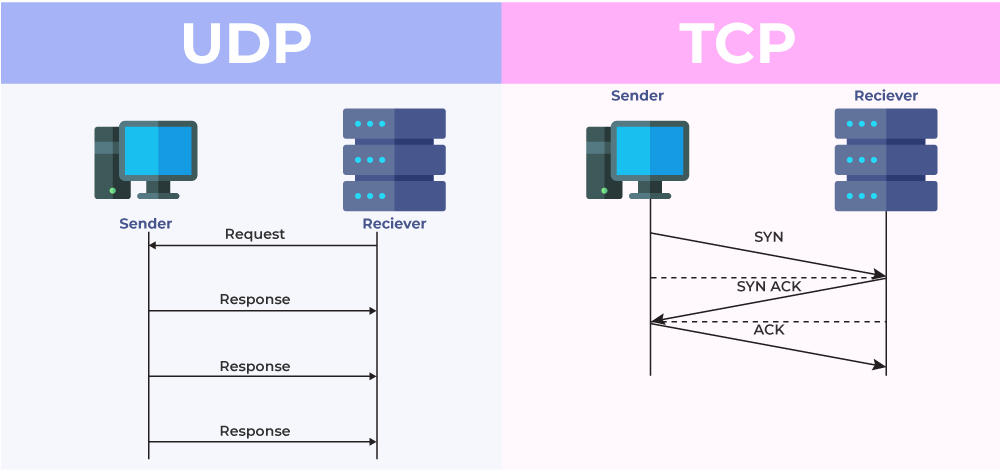
\includegraphics[width=1\textwidth]{figures/tcp_vs_udp_geeksforgeeks.png}
  \caption{Comparazione graficata tra i 2 protocolli. Immagine tratta da \cite{TCPvsUDP_geeksforgeeks}}
  \label{Comparazione graficata tra i 2 protocolli}
\end{figure}

\noindent Oltre a ciò TCP implementa meccanismi di controllo del flusso che evitano la congestione della rete, garantendo una comunicazione efficiente anche in condizioni di carico elevato.

\noindent Ovviamente per garantire questi aspetti, ci sono compromessi, \textbf{TCP} infatti è un protocollo sensibilmente più "pesante" rispetto ad \textbf{UDP}. Nonostante la latenza di TCP, si è deciso di sfruttare il protocollo MQTT per l'affidabilità nella trasmissione. Questa scelta è stata dettata dalla necessità di garantire la consegna dei messaggi in modo sicuro e ordinato, anche in condizioni di rete instabili.

\subsection{Sicurezza}
\noindent Nell'ambito dell'analisi di scenari di rete pubblica come il nostro, l'aspetto della sicurezza riveste un'importanza cruciale. In tale contesto, l'adozione di ROS per la guida remota potrebbe rivelarsi una scelta non ottimale.

\noindent ROS, nella sua configurazione standard, non prevede l'implementazione di meccanismi di sicurezza a livello di pacchetto. Di conseguenza, i dati scambiati tra i nodi della rete vengono trasmessi in chiaro, rendendoli potenzialmente accessibili a qualsiasi entità connessa alla rete. Questa vulnerabilità espone i sistemi a rischi di intercettazione, manipolazione o alterazione dei dati, con potenziali conseguenze negative sulla privacy e sulla sicurezza operativa.

\noindent Al contrario MQTT supporta nativamente lo strato di trasporto sicuro SSL/TLS, che fornisce una crittografia end-to-end dei dati scambiati tra i dispositivi. Questo significa che anche in caso di intercettazione delle comunicazioni, i dati rimarranno incomprensibili agli intrusi.

\subsection{Struttura}
Nell'ambito della guida remota, la resilienza del sistema è un fattore critico. Un'infrastruttura deve essere in grado di operare in modo affidabile anche in condizioni avverse, garantendo la continuità del servizio e la sicurezza dei dati. In questo contesto, MQTT dimostra una maggiore resilienza rispetto a ROS. 

\noindent MQTT è progettato per operare in ambienti distribuiti, con molti dispositivi connessi a un broker centrale. Questa architettura rende il sistema più resistente a guasti locali, poiché la perdita di un singolo dispositivo o di una connessione non compromette necessariamente l'intero sistema.

\noindent Al contrario ROS spesso si basa su un unico organo, chiamato \textit{ROS Master} che coordina tutte le comunicazioni. La perdita o l'irraggiungibilità di questo organo può causare il blocco dell'intero sistema.

\begin{figure}[H]
  \centering
  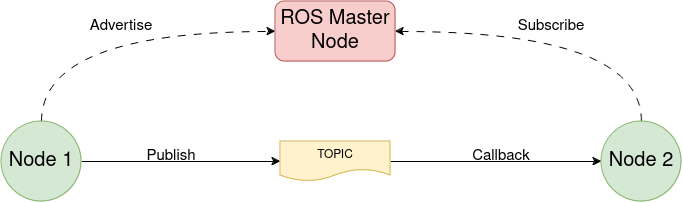
\includegraphics[width=1\textwidth]{figures/ros_master.png}
  \caption{Struttura del sistema ROS}
  \label{struttura_ros}
\end{figure}

\subsection{Controllo del QOS}
Un'ulteriore punto da considerare è quella della gestione della \textbf{QOS} (Quality Of Service). Il concetto di \textbf{QOS}indica il livello di garanzia che una rete offre per quanto riguarda la consegna dei dati. Una bassa Quality Of Service indica che i pacchetti non vengono consegnati correttamente o che addirittura non è certa la ricezione di questi messaggi.  

\noindent Entrambi i protocolli offrono meccanismi di gestione della \textbf{QOS}, nello specifico.

\noindent \textbf{MQTT} offre tre livelli di gestione (0, 1, 2) che consentono di adattare il livello di affidabilità della rete, tutti e tre i livelli si basano sul come e quante volte il messaggio deve essere riinviato perchè questo possa essere considerato ricevuto. 

\begin{itemize}
  \item \textit{QoS 0} (At most once): Il messaggio viene consegnato al massimo una volta. Non c'è alcuna garanzia di consegna, e il messaggio potrebbe perdersi. È il livello più veloce ma meno affidabile
  \item \textit{QoS 1} (At least once): Il messaggio viene consegnato almeno una volta. Il broker invia un messaggio di conferma al publisher, e se non riceve conferma, reinvia il messaggio. Questo livello garantisce che il messaggio arrivi, ma potrebbe arrivare più di una volta
  \item \textit{QoS 2} (Exactly once): Il messaggio viene consegnato esattamente una volta. Il broker invia un messaggio di conferma al publisher, e solo dopo aver ricevuto questa conferma, considera il messaggio consegnato. Questo è il livello più affidabile ma anche il più lento
\end{itemize}

\noindent \textbf{ROS} invece, non offre un meccanismo di QoS così definito e flessibile come MQTT. La gestione della qualità del servizio in ROS è più legata alla configurazione dei nodi e dei topic, e spesso richiede una implementazione personalizzata per garantire un livello di affidabilità specifico. 

Le possibili configurazioni che è possibile fare sui nodi ROS sono:
\begin{itemize}
  \item \textit{History}: Definisce la quantità di dati che possono essere memorizzati in un buffer prima che vengano scartati.
  \item \textit{Depth}: Indica la dimensione massima del buffer.
  \item \textit{Reliability}: Determina il livello di affidabilità della comunicazione (best-effort, reliable, etc.).
  \item \textit{Durability}: Specifica se i dati devono essere persistenti anche se i nodi non sono connessi.
  \item \textit{Liveliness}: Definisce come spesso un nodo deve dimostrare di essere attivo.
\end{itemize}
